\section{Scalar Field Visualization} % (fold)
\label{sec:scalar_fields}
%
A scalar field is a map $s(\vx, t): D \times T \mapsto \RRSet$ that assigns a
scalar value to each position $\vx$ and time $t$ in spatial and temporal domains
$D$ and $T$.
%
The spatial domain $D$ is a subset of the (two- or three-dimensional) Euclidean
space $\EESet^n$.
%
The temporal domain $T$ is usually an interval of $\RRSet$.
%
Examples of scalar fields are the temperature in a solid object, the population
density on a map, and the attenuation coefficient in a \ac{CT} scan.
%
If the scalar field does not change with time, or we are only interested in a
single instant, we often just write $s(\vx)$ and omit the time parameter.
%

% \subsection{Visualization Methods for Scalar Fields} % (fold)
% \label{sub:visualization_methods_for_scalar_fields}
%
% \begin{itemize}
%     \item Space-filling
%     \begin{itemize}
%         \item Colormapping (2D)
%         \item Height-mapping (2D)
%         \item Direct Volume rendering (3D)
%     \end{itemize}
%     \item Geometry-based
%     \begin{itemize}
%         \item Isocontours/surfaces (cite marching cubes)
%         \item maxima/minima/saddles
%         \item Morse-Smale-complex
%         \item Ridge lines/surfaces
%     \end{itemize}
% \end{itemize}
%
Methods for visualizing scalar fields can be roughly separated into two groups:
image-based and geometry-based.
%
We will briefly cover the most important methods in the following.
%
\Todo{add citations}
%

\subsection{Image-Based Methods} % (fold)
\label{sub:scalar_image_based}
%
Image-based methods map the scalar at each position in space to a property and
display it directly.
%
Among such methods are \emph{color-mapping} and \emph{height-mapping} for
\ac{2D} scalar fields as well as \emph{direct volume rendering} for \ac{3D}
scalar fields.
%

%
\subsubsection{Color-Mapping}
%
Color-mapping means assigning each scalar value a color from a
predefined color map and displaying the result as an image or texture.
%
Due to its simplicity, it is probably the most widespread method presented here.
%
This technique is only applicable to \ac{2D} scalar fields, but is commonly used
on \ac{3D} data by selecting slices or surfaces in a volume, or by displaying
the scalar value on the outside surface of the volume.
%
\begin{figure}[t]
    % \centering
    \begin{captionbeside}{Direct volume rendering of a \ac{CT} scan of a human skull using
        volumetric raycasting with gradient-based shading. Image source: Wi\-ki\-me\-di\-a
        Com\-mons.\label{fig:direct_volume_rendering}}
        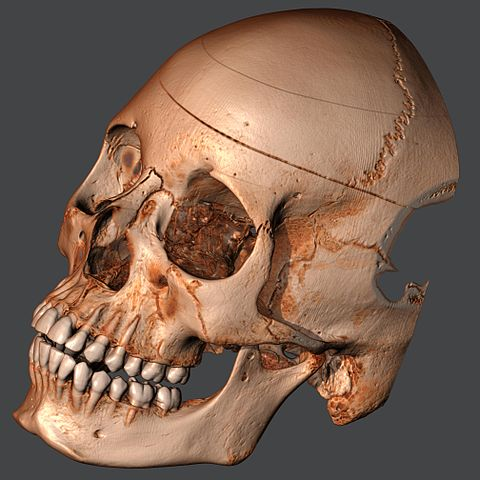
\includegraphics[width=0.6\textwidth]{figures/skull_direct_volume_rendering.jpg}
    \end{captionbeside}
\end{figure}
%

%
\subsubsection{Height-Mapping}
%
Height-mapping only works on \ac{2D} data.
%
It essentially means interpreting the scalar value at each point as a height
value and displaying the resulting three-dimensional surface.
%
Because it transforms \ac{2D} information into \ac{3D} information, it is best
suited for interactive settings, where the resulting surface can be rotated and
viewed from all directions.
%

%
\subsubsection{Direct Volume Rendering}
%
Direct volume rendering~\cite{Levoy1988,Drebin1988} is the extension of
color-mapping to \ac{3D} scalar fields.
%
It involves two steps: Applying a transfer function, and accumulating the
resulting colors and opacities along viewing rays to produce an image.
%
The transfer function has to be chosen carefully to reveal the structures in the
data that are interesting, and make the uninteresting parts transparent.
%
Color and opacity values are then accumulated along viewing rays to simulate the
transport of light through a semitransparent medium.
%

%
The shading of a solid surface can be approximated by using the gradient of the
scalar field as the surface normal (see \cref{fig:direct_volume_rendering}).
%
More advanced techniques use a two-dimensional transfer function that also takes
the gradient magnitude into account when deciding the color, opacity and
shading parameters of a point along the viewing ray~\cite{Kindlmann1998}.
%
% subsection scalar_image_based (end)

\subsection{Geometry-Based Methods} % (fold)
\label{sub:scalar_geometry_based}
%
Geometry-based methods extract some geometrical structures from the data and
display these structures.
%
\emph{Isocontours and -surfaces} belong in this category together with
topological features such as \emph{extremal- and saddle points}, as well as
\emph{ridge- and valley lines and -surfaces}.
%

%
\subsubsection{Isocontours and -surfaces}
%
Isocontours and -surfaces are subsets of the scalar field where the
scalar is equal to a constant (iso-) value.
%
In the literature these are also often referred to as \emph{level sets}.
%
They form lines or surfaces that are always closed or end at the domain
boundary, and that never intersect each other.
%
For \ac{2D} scalar fields, it is common to plot contours for several isovalues
at once, which resemble the height lines we know from maps.
%
In \ac{3D}, it is rare to display more than two or three different isosurfaces
at the same time due to occlusion problems.
%

%
\subsubsection{Critical Points}
%
Critical points are points in a scalar field where the gradient becomes zero.
%
As such, they are features of the scalar field's topology.
%
Critical points can be classified by the eigenvalues of the Hessian matrix at
the critical point:
%
If all eigenvalues are positive the point is a minimum, if all are negative it
is a maximum, and if the Hessian has both positive and negative eigenvalues,
the point is a saddle.
%

%
\subsubsection{Ridge- and Valley Lines and -Surfaces}
%
Ridge- and valley lines and -surfaces also belong to the category
of topological features.
%
There is no universal agreed-upon definition for these types of features.
%
The two most common, competing definitions are \emph{watersheds} and
\emph{height ridges}~\cite{Peikert2008,Eberly2012}.
%
Watersheds are global features that separate the scalar field into ``areas of
influence'' of the different minima (or maxima).
%
Imaginine a scalar field as a height field.
%
Starting a gradient descent from two points on the same side of a watershed
will end up in the same minimum.
%
Starting from two points on opposite sides of the watershed will end up in two
different minima.
%

%
Height ridges are defined by a local differential analysis of the scalar field.
%
As such, their computation is less costly, but they do not provide a
space-filling segmentation of the data.
%
Often, computation of raw ridges and valleys produces a lot of small and
insignificant features due to noise.
%
An additional filtering step~\cite{Peikert2008} can be applied to only keep the
most significant lines (see \cref{fig:ridge_valley_lines}).
%
\begin{figure}[t]
    \begin{captionbeside}
        {Filtered ridge and valley lines of a scalar field.
        Ridges are shown in red, valleys in blue. The scalar field is visualized
        using a combination of height mapping (to obtain the shading) and
        isocontours. Image source: Peikert and Sadlo~\cite{Peikert2008}.
        \label{fig:ridge_valley_lines}}
        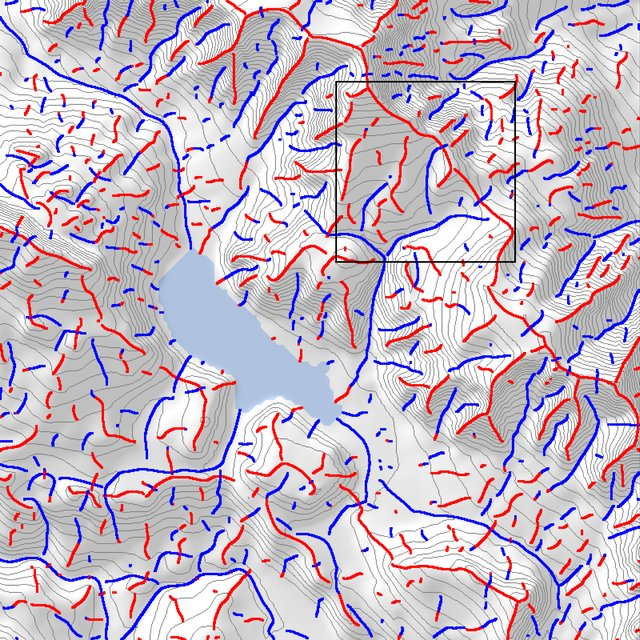
\includegraphics[width=0.6\textwidth]{figures/ridge_valley_lines_peikert.jpg}
    \end{captionbeside}
\end{figure}
%
\subsubsection{Morse-Smale Decomposition} % (fold)
\label{ssub:morse_smale_decomposition}
%
The Morse-Smale Decomposition forms the topological skeleton of a scalar field.
%
It is based on the idea of integral lines of the scalar field.
%
These are maximal paths that are everywhere tangent to the gradient of the
scalar field (see also integral curves in vector fields,
\cref{sub:integral_curves_and_surfaces}).
%
Integral lines always connect two critical points or end at the domain boundary.
%

%
The Morse-Smale decomposition separates the scalar field into a disjoint set of
cells whose union is the whole domain.
%
Each cell is defined as the set of all integral lines that connect the same
minimum and maximum.
%
In this sense, the Morse-Smale decomposition is closely related to the idea of
watersheds:
%
The boundarties of the cells are precisely the watersheds of the scalar field
and its negative.
%
% subsubsection morse_smale_decomposition (end)
%
% subsection scalar_geometry_based (end)
%
% subsection visualization_methods_for_scalar_fields (end)
%
% section scalar_fields (end)